%% ltee.tex
%% Author: Leighton Pritchard
%% Copyright: James Hutton Institute
%% Example slides: The Long-Term Evolution Experiment

%
\begin{frame}
  \frametitle{\textit{E. coli} LTEE
                   \footnote{\tiny{\href{http://dx.doi.org/10.1016/j.jmb.2009.09.052
}{Jeong \textit{et al}. (2009) \textit{J. Mol. Biol.} doi:10.1016/j.jmb.2009.09.052
}}}
                   \footnote{\tiny{\href{http://dx.doi.org/10.1038/nature08480
}{Barrick \textit{et al}. (2009) \textit{Nature} doi:10.1038/nature08480
}}}
                   \footnote{\tiny{\href{http://dx.doi.org/10.1126/science.1243357
}{Wiser \textit{et al}. (2013) \textit{Science} doi:10.1126/science.1243357
}}}}
    \begin{columns}[c] 
      \column{.6\textwidth} 
        \begin{itemize}
          \item \textcolor{RawSienna}{Run by the Lenski lab, Michigan State University since 1988 \\
          (\href{http://myxo.css.msu.edu/ecoli/}{http://myxo.css.msu.edu/ecoli/})}
          \item \textcolor{hutton_green}{12 flasks, citrate usage selection}
          \item \textcolor{hutton_blue}{$>$50,000 generations of \textit{E coli}!}
          \begin{itemize}
            \item Cultures propagated every day
            \item Every 500 generations (75 days), mixed-population samples stored
            \item Mean fitness estimated at 500 generation intervals
          \end{itemize}
        \end{itemize}
      \column{.4\textwidth}
        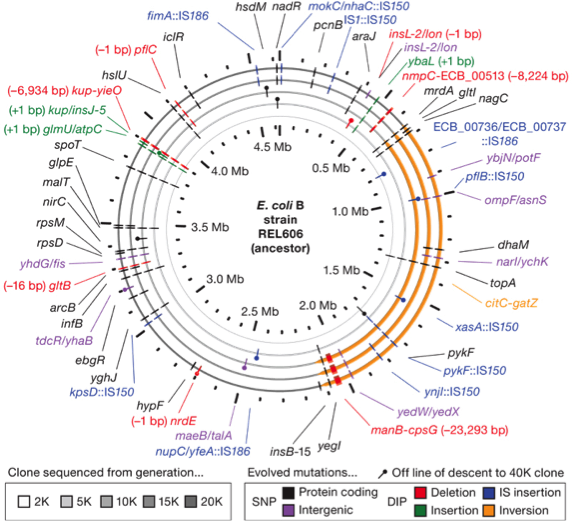
\includegraphics[width=\textwidth]{images/ltee_circular} \\
        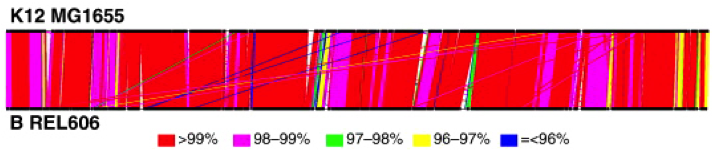
\includegraphics[width=\textwidth]{images/ltee_linear}        
    \end{columns}  
\end{frame}